\subsection{Problem~3}%
\label{problem:3}

Estimate the exact solution to the following system of linear equations using Gaussian elimination:
\begin{equation*}
    \systeme{0.835x_1 + 0.667x_2 = 0.168,0.333x_1 + 0.266x_2 = 0.067}
\end{equation*}
The slightly perturb $b_2$ from $0.067$ to $0.066$ and compute iterative approximations to the perturbed system using the selected iterative solvers.
Draw the distance between the exact solution and the iterative approximations versus iterations.
Start the iteration from $x_1^{(0)}=x_2^{(0)}=0$.
Estimate the computational costs for each tested methods and compare them with the costs for the Gaussian elimination.

\subsubsection*{Mathematics}
Following the manual calculations of the Gaussian elimination, we transform the augmented matrix
to the upper triangular form:
\begin{equation*}
\begin{split}
    \begin{amatrix}{1}{1}
        \matr{A} & \matr{b}
    \end{amatrix} =
    \begin{amatrix}{2}{1}
    0.835 & 0.6670 & 0.168\\
    0.333 & 0.266 & 0.067
    \end{amatrix}&\xrightarrow{R_2 - \frac{0.333}{0.835}R_1}
    \begin{amatrix}{2}{1}
    0.835 & 0.667 & 0.168\\
    0 & 0 & 0
    \end{amatrix}
\end{split}
\end{equation*}
The second equation reduces to $0x_1+0x_2=0$, which its always true. This implies that the system have infinitely many solutions. To express the exact solution we can solve the first equation by treating the value of $x_2$ as free variable.

Performing back substitution, we obtained:
\begin{equation*}
  \begin{split}
  \systeme{0.835x_1 + 0.667x_2 = 0.168,
  0x_1 + 0x_2 =0}\rightarrow
  \begin{cases}
    x_1=\phantom{-}1\\
    x_2=-1\\
    \end{cases}
  \end{split}
\end{equation*}
Afterwards, we perturb$b_2$ form $0.067$ to $0.066$, and again apply Gaussian elimination:
\begin{equation*}
\begin{split}
    \begin{amatrix}{1}{1}
        \matr{A} & \matr{b}
    \end{amatrix} =
    \begin{amatrix}{2}{1}
    0.835 & 0.6670 & 0.168\\
    0.333 & 0.266 & 0.066
    \end{amatrix}&\xrightarrow{R_2 - \frac{0.333}{0.835}R_1}
    \begin{amatrix}{2}{1}
    0.835 & 0.667 & 0.168\\
    0 & -0 & 0.001
    \end{amatrix}
\end{split}
\end{equation*}
In this case the second equation becomes $0x_1+0x_2=0.001$ which gives us inconsistent solution. After performing back substitution:
\begin{equation*}
  \begin{split}
  \systeme{0.835x_1 + 0.667x_2 = 0.168,
  0x_1 + 0x_2 =0.001}\rightarrow
  \begin{cases}
    x_1=-666\\
    x_2=\phantom{-}834\\
    \end{cases}
  \end{split}
\end{equation*}

The extremal change in the solution value indicates that the system is ill-conditioned.

\subsubsection*{Solution}
For slightly changed system we compute iterative approximation using the Kaczmarz(\ref{alg:kaczmarz}) and SOR(\ref{alg:sor}) methods:

\lstinputlisting[style=Matlab-editor, breaklines=false]{problems/problem_3.m}

The results shows that the iterative methods provides more stable approximations compared to Gaussian elimination. The following table summarize the computed solution:

\begin{table}[h]
    \centering
    \begin{tabular}{c|c|c|c}
         Method& Gaussian elimination  & Kaczmarz & SOR\\
         \hline
         $x_1$ & -666 & 0.1210 & 0.2328\\
         \hline
         $x_2$ & \phantom{-}834& 0.0967 & -0.0420\\
    \end{tabular}
    \caption{Calculated results using MATLAB of perturbed system}
    \label{tab:tablele}
\end{table}

\begin{figure}[ht]
    \centering
    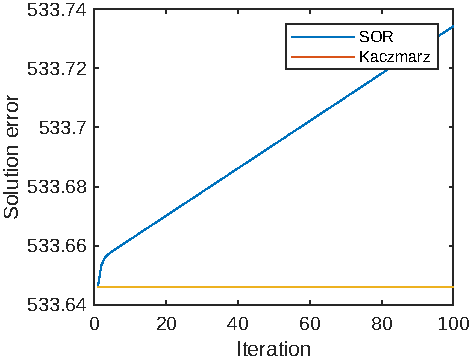
\includegraphics[width=0.75\linewidth]{figures/Figure_problem_3_b.pdf}
    \caption{Solution error $e$ vs iterations k for the perturbed system for tested method in \ref{problem:3}}
    \label{fig:enter-label}
\end{figure}
\vspace{0.2\linewidth}
For comparison, we also solve the original system using iterative methods:


\begin{table}[h]
    \centering
    \begin{tabular}{c|c|c|c}
         Method& Gaussian elimination  & Kaczmarz & SOR\\
         \hline
         $x_1$ & \phantom{-}1 & 0.1228 & 0.1340\\
         \hline
         $x_2$ & -1 & 0.0981 & 0.0841\\
    \end{tabular}
    \caption{Calculated results using MATLAB of original system}
    \label{tab:tablele}
\end{table}

\begin{figure}[h]
    \centering
    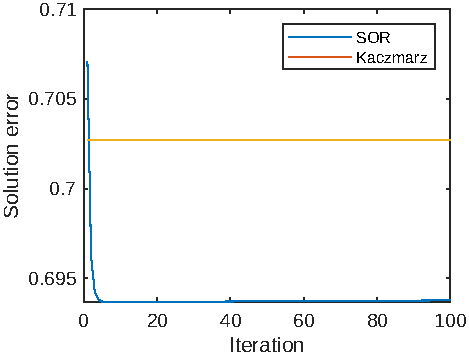
\includegraphics[width=0.75\linewidth]{figures/Figure_problem_3.pdf}
    \caption{The graph of distance between the exact and the approximate solutions versus iterations of original system.}
    \label{fig:enter-label}
\end{figure}
To summarize from the results we noticed that the system is highly sensitive to small perturbations. Kaczmarz method showing better resistance to perturbation.
